\documentclass{ximera}

%\usepackage{todonotes}

\newcommand{\todo}{}

\usepackage{esint} % for \oiint
\ifxake%%https://math.meta.stackexchange.com/questions/9973/how-do-you-render-a-closed-surface-double-integral
\renewcommand{\oiint}{{\large\bigcirc}\kern-1.56em\iint}
\fi


\graphicspath{
  {./}
  {ximeraTutorial/}
  {basicPhilosophy/}
  {functionsOfSeveralVariables/}
  {normalVectors/}
  {lagrangeMultipliers/}
  {vectorFields/}
  {greensTheorem/}
  {shapeOfThingsToCome/}
  {dotProducts/}
  {../productAndQuotientRules/exercises/}
  {../normalVectors/exercisesParametricPlots/}
  {../continuityOfFunctionsOfSeveralVariables/exercises/}
  {../partialDerivatives/exercises/}
  {../chainRuleForFunctionsOfSeveralVariables/exercises/}
  {../commonCoordinates/exercisesCylindricalCoordinates/}
  {../commonCoordinates/exercisesSphericalCoordinates/}
  {../greensTheorem/exercisesCurlAndLineIntegrals/}
  {../greensTheorem/exercisesDivergenceAndLineIntegrals/}
  {../shapeOfThingsToCome/exercisesDivergenceTheorem/}
  {../greensTheorem/}
  {../shapeOfThingsToCome/}
}

\newcommand{\mooculus}{\textsf{\textbf{MOOC}\textnormal{\textsf{ULUS}}}}

\usepackage{tkz-euclide}\usepackage{tikz}
\usepackage{tikz-cd}
\usetikzlibrary{arrows}
\tikzset{>=stealth,commutative diagrams/.cd,
  arrow style=tikz,diagrams={>=stealth}} %% cool arrow head
\tikzset{shorten <>/.style={ shorten >=#1, shorten <=#1 } } %% allows shorter vectors

\usetikzlibrary{backgrounds} %% for boxes around graphs
\usetikzlibrary{shapes,positioning}  %% Clouds and stars
\usetikzlibrary{matrix} %% for matrix
\usepgfplotslibrary{polar} %% for polar plots
\usepgfplotslibrary{fillbetween} %% to shade area between curves in TikZ
\usetkzobj{all}
%\usepackage[makeroom]{cancel} %% for strike outs
%\usepackage{mathtools} %% for pretty underbrace % Breaks Ximera
%\usepackage{multicol}
\usepackage{pgffor} %% required for integral for loops



%% http://tex.stackexchange.com/questions/66490/drawing-a-tikz-arc-specifying-the-center
%% Draws beach ball
\tikzset{pics/carc/.style args={#1:#2:#3}{code={\draw[pic actions] (#1:#3) arc(#1:#2:#3);}}}



\usepackage{array}
\setlength{\extrarowheight}{+.1cm}   
\newdimen\digitwidth
\settowidth\digitwidth{9}
\def\divrule#1#2{
\noalign{\moveright#1\digitwidth
\vbox{\hrule width#2\digitwidth}}}





\newcommand{\RR}{\mathbb R}
\newcommand{\R}{\mathbb R}
\newcommand{\N}{\mathbb N}
\newcommand{\Z}{\mathbb Z}

\newcommand{\sagemath}{\textsf{SageMath}}


%\renewcommand{\d}{\,d\!}
\renewcommand{\d}{\mathop{}\!d}
\newcommand{\dd}[2][]{\frac{\d #1}{\d #2}}
\newcommand{\pp}[2][]{\frac{\partial #1}{\partial #2}}
\renewcommand{\l}{\ell}
\newcommand{\ddx}{\frac{d}{\d x}}

\newcommand{\zeroOverZero}{\ensuremath{\boldsymbol{\tfrac{0}{0}}}}
\newcommand{\inftyOverInfty}{\ensuremath{\boldsymbol{\tfrac{\infty}{\infty}}}}
\newcommand{\zeroOverInfty}{\ensuremath{\boldsymbol{\tfrac{0}{\infty}}}}
\newcommand{\zeroTimesInfty}{\ensuremath{\small\boldsymbol{0\cdot \infty}}}
\newcommand{\inftyMinusInfty}{\ensuremath{\small\boldsymbol{\infty - \infty}}}
\newcommand{\oneToInfty}{\ensuremath{\boldsymbol{1^\infty}}}
\newcommand{\zeroToZero}{\ensuremath{\boldsymbol{0^0}}}
\newcommand{\inftyToZero}{\ensuremath{\boldsymbol{\infty^0}}}



\newcommand{\numOverZero}{\ensuremath{\boldsymbol{\tfrac{\#}{0}}}}
\newcommand{\dfn}{\textbf}
%\newcommand{\unit}{\,\mathrm}
\newcommand{\unit}{\mathop{}\!\mathrm}
\newcommand{\eval}[1]{\bigg[ #1 \bigg]}
\newcommand{\seq}[1]{\left( #1 \right)}
\renewcommand{\epsilon}{\varepsilon}
\renewcommand{\phi}{\varphi}


\renewcommand{\iff}{\Leftrightarrow}

\DeclareMathOperator{\arccot}{arccot}
\DeclareMathOperator{\arcsec}{arcsec}
\DeclareMathOperator{\arccsc}{arccsc}
\DeclareMathOperator{\si}{Si}
\DeclareMathOperator{\scal}{scal}
\DeclareMathOperator{\sign}{sign}


%% \newcommand{\tightoverset}[2]{% for arrow vec
%%   \mathop{#2}\limits^{\vbox to -.5ex{\kern-0.75ex\hbox{$#1$}\vss}}}
\newcommand{\arrowvec}[1]{{\overset{\rightharpoonup}{#1}}}
%\renewcommand{\vec}[1]{\arrowvec{\mathbf{#1}}}
\renewcommand{\vec}[1]{{\overset{\boldsymbol{\rightharpoonup}}{\mathbf{#1}}}}
\DeclareMathOperator{\proj}{\vec{proj}}
\newcommand{\veci}{{\boldsymbol{\hat{\imath}}}}
\newcommand{\vecj}{{\boldsymbol{\hat{\jmath}}}}
\newcommand{\veck}{{\boldsymbol{\hat{k}}}}
\newcommand{\vecl}{\vec{\boldsymbol{\l}}}
\newcommand{\uvec}[1]{\mathbf{\hat{#1}}}
\newcommand{\utan}{\mathbf{\hat{t}}}
\newcommand{\unormal}{\mathbf{\hat{n}}}
\newcommand{\ubinormal}{\mathbf{\hat{b}}}

\newcommand{\dotp}{\bullet}
\newcommand{\cross}{\boldsymbol\times}
\newcommand{\grad}{\boldsymbol\nabla}
\newcommand{\divergence}{\grad\dotp}
\newcommand{\curl}{\grad\cross}
%\DeclareMathOperator{\divergence}{divergence}
%\DeclareMathOperator{\curl}[1]{\grad\cross #1}
\newcommand{\lto}{\mathop{\longrightarrow\,}\limits}

\renewcommand{\bar}{\overline}

\colorlet{textColor}{black} 
\colorlet{background}{white}
\colorlet{penColor}{blue!50!black} % Color of a curve in a plot
\colorlet{penColor2}{red!50!black}% Color of a curve in a plot
\colorlet{penColor3}{red!50!blue} % Color of a curve in a plot
\colorlet{penColor4}{green!50!black} % Color of a curve in a plot
\colorlet{penColor5}{orange!80!black} % Color of a curve in a plot
\colorlet{penColor6}{yellow!70!black} % Color of a curve in a plot
\colorlet{fill1}{penColor!20} % Color of fill in a plot
\colorlet{fill2}{penColor2!20} % Color of fill in a plot
\colorlet{fillp}{fill1} % Color of positive area
\colorlet{filln}{penColor2!20} % Color of negative area
\colorlet{fill3}{penColor3!20} % Fill
\colorlet{fill4}{penColor4!20} % Fill
\colorlet{fill5}{penColor5!20} % Fill
\colorlet{gridColor}{gray!50} % Color of grid in a plot

\newcommand{\surfaceColor}{violet}
\newcommand{\surfaceColorTwo}{redyellow}
\newcommand{\sliceColor}{greenyellow}




\pgfmathdeclarefunction{gauss}{2}{% gives gaussian
  \pgfmathparse{1/(#2*sqrt(2*pi))*exp(-((x-#1)^2)/(2*#2^2))}%
}


%%%%%%%%%%%%%
%% Vectors
%%%%%%%%%%%%%

%% Simple horiz vectors
\renewcommand{\vector}[1]{\left\langle #1\right\rangle}


%% %% Complex Horiz Vectors with angle brackets
%% \makeatletter
%% \renewcommand{\vector}[2][ , ]{\left\langle%
%%   \def\nextitem{\def\nextitem{#1}}%
%%   \@for \el:=#2\do{\nextitem\el}\right\rangle%
%% }
%% \makeatother

%% %% Vertical Vectors
%% \def\vector#1{\begin{bmatrix}\vecListA#1,,\end{bmatrix}}
%% \def\vecListA#1,{\if,#1,\else #1\cr \expandafter \vecListA \fi}

%%%%%%%%%%%%%
%% End of vectors
%%%%%%%%%%%%%

%\newcommand{\fullwidth}{}
%\newcommand{\normalwidth}{}



%% makes a snazzy t-chart for evaluating functions
%\newenvironment{tchart}{\rowcolors{2}{}{background!90!textColor}\array}{\endarray}

%%This is to help with formatting on future title pages.
\newenvironment{sectionOutcomes}{}{} 



%% Flowchart stuff
%\tikzstyle{startstop} = [rectangle, rounded corners, minimum width=3cm, minimum height=1cm,text centered, draw=black]
%\tikzstyle{question} = [rectangle, minimum width=3cm, minimum height=1cm, text centered, draw=black]
%\tikzstyle{decision} = [trapezium, trapezium left angle=70, trapezium right angle=110, minimum width=3cm, minimum height=1cm, text centered, draw=black]
%\tikzstyle{question} = [rectangle, rounded corners, minimum width=3cm, minimum height=1cm,text centered, draw=black]
%\tikzstyle{process} = [rectangle, minimum width=3cm, minimum height=1cm, text centered, draw=black]
%\tikzstyle{decision} = [trapezium, trapezium left angle=70, trapezium right angle=110, minimum width=3cm, minimum height=1cm, text centered, draw=black]


\outcome{State the definition of the curl of a vector field in two dimensions.}
\outcome{State the definition of the curl of a vector field in three dimensions.}
\outcome{Understand how curl measures local rotation in two dimensions.}
\outcome{Understand that curl need not measure gobal rotation.}
\outcome{State Green's Theorem.}
\outcome{View Green's Theorem as a fundamental theorem of calculus.}

\title[Dig-In:]{Curl and Green's Theorem}

\begin{document}
\begin{abstract}
Green's Theorem is a fundamental theorem of calculus.
\end{abstract}
\maketitle

In this section we will learn the \textit{fundamental derivative} for
vector fields, as well as a new fundamental theorem of calculus.


\section{The curl of a vector field}


Calculus has taught us that knowing the derivative of a function
$f:\R\to\R$ can tell us important information about the function.  In
a similar way we have that seen that if we wish to understand a
function of several variables $F:\R^n\to\R$, then the gradient, $\grad
F$, contains similar useful information. If you have a vector field
\[
\vec{F}:\R^n\to\R^n,
\]
we now ask: ``what is the natural analogue of a derivative in this
setting?'' When the vector field is two or three-dimensional, the
\textit{curl} is the analogue of the derivative that we are looking
for:


\begin{definition}\index{scalar curl}
  In two dimensions, given a vector field $\vec{F}:\R^2\to \R^2$, where
  \[
  \vec{F}(x,y) = \vector{M(x,y),N(x,y)}
  \]
  the (scalar) \dfn{curl} is given by
  \[
  \curl \vec F = \pp[N]{x}-\pp[M]{y}.
  \]
  In three dimensions, given a vector field $\vec{F}:\R^3\to\R^3$, where
  \[
  \vec{F}(x,y,z) = \vector{U(x,y,z)),V(x,y,z)),W(x,y,z)}
  \]
  the \dfn{curl} is given by
  \begin{align*}
  \curl \vec F &= \det
  \begin{bmatrix}
    \veci & \vecj & \veck \\
    \pp{x} & \pp{y} & \pp{z}\\
    U & V & W
  \end{bmatrix}\\
  &= \veci\left(\pp[W]{y}-\pp[V]{z}\right)-
  \vecj\left(\pp[W]{x}-\pp[U]{z}\right)+
  \veck\left(\pp[V]{x}-\pp[U]{y}\right).
  \end{align*}
  Other authors sometimes use the notation $\mathop{\mathrm{rot}}\vec{F}$ for
  the scalar curl of a two-dimensional vector field $\vec{F}:\R^2\to
  \R^2$, and $\mathop{\mathrm{curl}}\vec{F}$ for the curl of a
  three-dimensional vector field $\vec{F}:\R^3\to\R^3$.
\end{definition}


\begin{question}
  In two dimensions, is $\curl\vec{F}$ a number or a vector?
  \begin{prompt}
  \begin{multipleChoice}
    \choice[correct]{number.}
    \choice{vector.}
  \end{multipleChoice}
  \end{prompt}
  \begin{question}
    In three dimensions, is $\curl\vec{F}$ a number or a vector?
    \begin{prompt}
      \begin{multipleChoice}
        \choice{number.}
        \choice[correct]{vector.}
      \end{multipleChoice}
    \end{prompt}
    \end{question}
\end{question}


\begin{question}
  Consider the vector field $\vec{F}(x,y) = \vector{-y,x}$. Compute:
  \[
  \curl\vec{F}(x,y) \begin{prompt}= \answer{2}\end{prompt}
  \]
  \begin{question}
    Consider the vector field $\vec{F}(x,y,z) = \vector{-z,x,y}$. Compute:
    \[
    \curl\vec{F}(x,y,z)   \begin{prompt}
      = \vector{\answer{1},\answer{-1},\answer{1}}
    \end{prompt}
    \]
  \end{question}
\end{question}

Now for something you've seen before, but in a different form.

\begin{question}
  Let $F:\R^2\to\R$. Compute:
  \[
  \curl\grad F(x,y) \begin{prompt}= \answer{0}\end{prompt}
  \]
  \begin{question}
    Let $F:\R^3\to\R$. Compute:
    \[
    \curl\grad F(x,y,z) \begin{prompt}= \vector{\answer{0},\answer{0},\answer{0}}\end{prompt}
    \] 
  \end{question}
\end{question}

\begin{question}
  When $\curl\vec{F} = \vec{0}$, then you know:
  \begin{selectAll}
    \choice[correct]{$\vec{F}$ is a gradient field.}
    \choice[correct]{$\vec{F}$ is a conservative field.}
    \choice[correct]{$\vec{F}:\R^3\to\R^3$.}
  \end{selectAll}
  \begin{feedback}
    You can be assured that $\vec{F}:\R^3\to\R^3$, since $\vec{0}$ is
    a vector. We only know a definition for curl in two and three
    dimensions; however, the two-dimensional definition is a scalar,
    not a vector. So if $\curl\vec{F} = \vec{0}$, then
    $\vec{F}:\R^3\to\R^3$.
  \end{feedback}
\end{question}


\subsection{What does the curl measure?}


The curl of a vector field measures the rate that the direction of
field vectors ``twist'' as $x$ and $y$ change. Imagine the vectors in
a vector field as representing the current of a river. A positive curl
at a point tells you that a ``beach-ball'' floating at the point would
be rotating in a counterclockwise direction. A negative curl at a
point tells you that a ``beach-ball'' floating at the point would be
rotating in a clockwise direction. Zero curl means that the
``beach-ball'' would not be rotating. Below we see our ``beach-ball''
with two field vectors. If $\vec{F}(x,y) = \vector{M(x,y),N(x,y)}$
\begin{image}
  \begin{tikzpicture}%[framed]
    \begin{axis}[
        hide axis,
        width=2in,
        height=2in,
	ymin=-.9,ymax=.7,
	xmin=-.8,xmax=.8,
      ]
       \addplot[penColor2,thick,->] coordinates{
                (-.6,0) (-.6,.3) 
       };
       \addplot[penColor2,thick,->] coordinates{
                (.6,0) (.6,.7) 
       };


       \addplot[penColor, ultra thick, domain=0:360,smooth] ({.5*cos(x)},{.5*sin(x)});

       \addplot[penColor, ultra thick, domain=0:360,smooth] ({.2*cos(x)},{.2*sin(x)});

       \addplot[penColor, ultra thick] coordinates{
       ({.2*cos(45)},{.2*sin(45)}) ({.5*cos(45)},{.5*sin(45)})
       };

       \addplot[penColor, ultra thick] coordinates{
       ({.2*cos(135)},{.2*sin(135)}) ({.5*cos(135)},{.5*sin(135)})
       };

       \addplot[penColor, ultra thick] coordinates{
       ({.2*cos(225)},{.2*sin(225)}) ({.5*cos(225)},{.5*sin(225)})
       };

       \addplot[penColor, ultra thick] coordinates{
       ({.2*cos(315)},{.2*sin(315)}) ({.5*cos(315)},{.5*sin(315)})
       };
       \addplot[penColor, ultra thick,domain=364:365,->] ({.5*cos(x)},{.5*sin(x)});
       %\draw[penColor, ultra thick,->] (axis cs: .49,-.1) -- (axis cs: .5,.1);
       
       \node[inner sep=0pt,text width=6cm,scale=.5] at (axis cs: 0,-.7) {
         \footnotesize Since the length of the field vector increases
         as we increase $x$, we see that $\pp[N]{x} > 0$.};

    \end{axis}
  \end{tikzpicture}
\end{image}
we see that the right field vector is larger than the left, thus
giving the ``beach-ball'' a counterclockwise rotation.  In an entirely
similar way, if we have
\begin{image}
  \begin{tikzpicture}%[framed]
    \begin{axis}[
        hide axis,
        width=2in,
        height=2in,
	ymin=-.9,ymax=.7,
	xmin=-.8,xmax=.8,
      ]
       \addplot[penColor2,thick,->] coordinates{
                (0,.6) (.3,.6) 
       };
       \addplot[penColor2,thick,->] coordinates{
                (0,-.6) (.7,-.6) 
            };


       \addplot[penColor, ultra thick, domain=0:360,smooth] ({.5*cos(x)},{.5*sin(x)});

       \addplot[penColor, ultra thick, domain=0:360,smooth] ({.2*cos(x)},{.2*sin(x)});

       \addplot[penColor, ultra thick] coordinates{
       ({.2*cos(45)},{.2*sin(45)}) ({.5*cos(45)},{.5*sin(45)})
       };

       \addplot[penColor, ultra thick] coordinates{
       ({.2*cos(135)},{.2*sin(135)}) ({.5*cos(135)},{.5*sin(135)})
       };

       \addplot[penColor, ultra thick] coordinates{
       ({.2*cos(225)},{.2*sin(225)}) ({.5*cos(225)},{.5*sin(225)})
       };

       \addplot[penColor, ultra thick] coordinates{
       ({.2*cos(315)},{.2*sin(315)}) ({.5*cos(315)},{.5*sin(315)})
       };

       \addplot[penColor, ultra thick,domain=364:365,->] ({.5*cos(x)},{.5*sin(x)});
       %\draw[penColor, ultra thick,->] (axis cs: .49,-.1) -- (axis cs: .5,.1) ;
       \node[inner sep=0pt,text width=6cm,scale=.5] at (axis cs: 0,-.75) {

        \footnotesize Since the length of the field vector decreases
        as we increase $y$, we see that $-\pp[M]{y} > 0$.};
    \end{axis}
  \end{tikzpicture}
\end{image}
we see that the bottom field vector is larger than the top, thus
giving the ``beach-ball'' a counterclockwise rotation. Thus the curl
combines $\pp[N]{x}$ and $-\pp[M]{y}$
\[
\curl\vec{F} = \pp[N]{x} - \pp[M]{y}
\]
to obtain the local rotation of the field. The most obvious
example of a vector field with nonzero curl is $\vec{F}(x,y) =
\vector{-y,x}$.
\begin{image}
  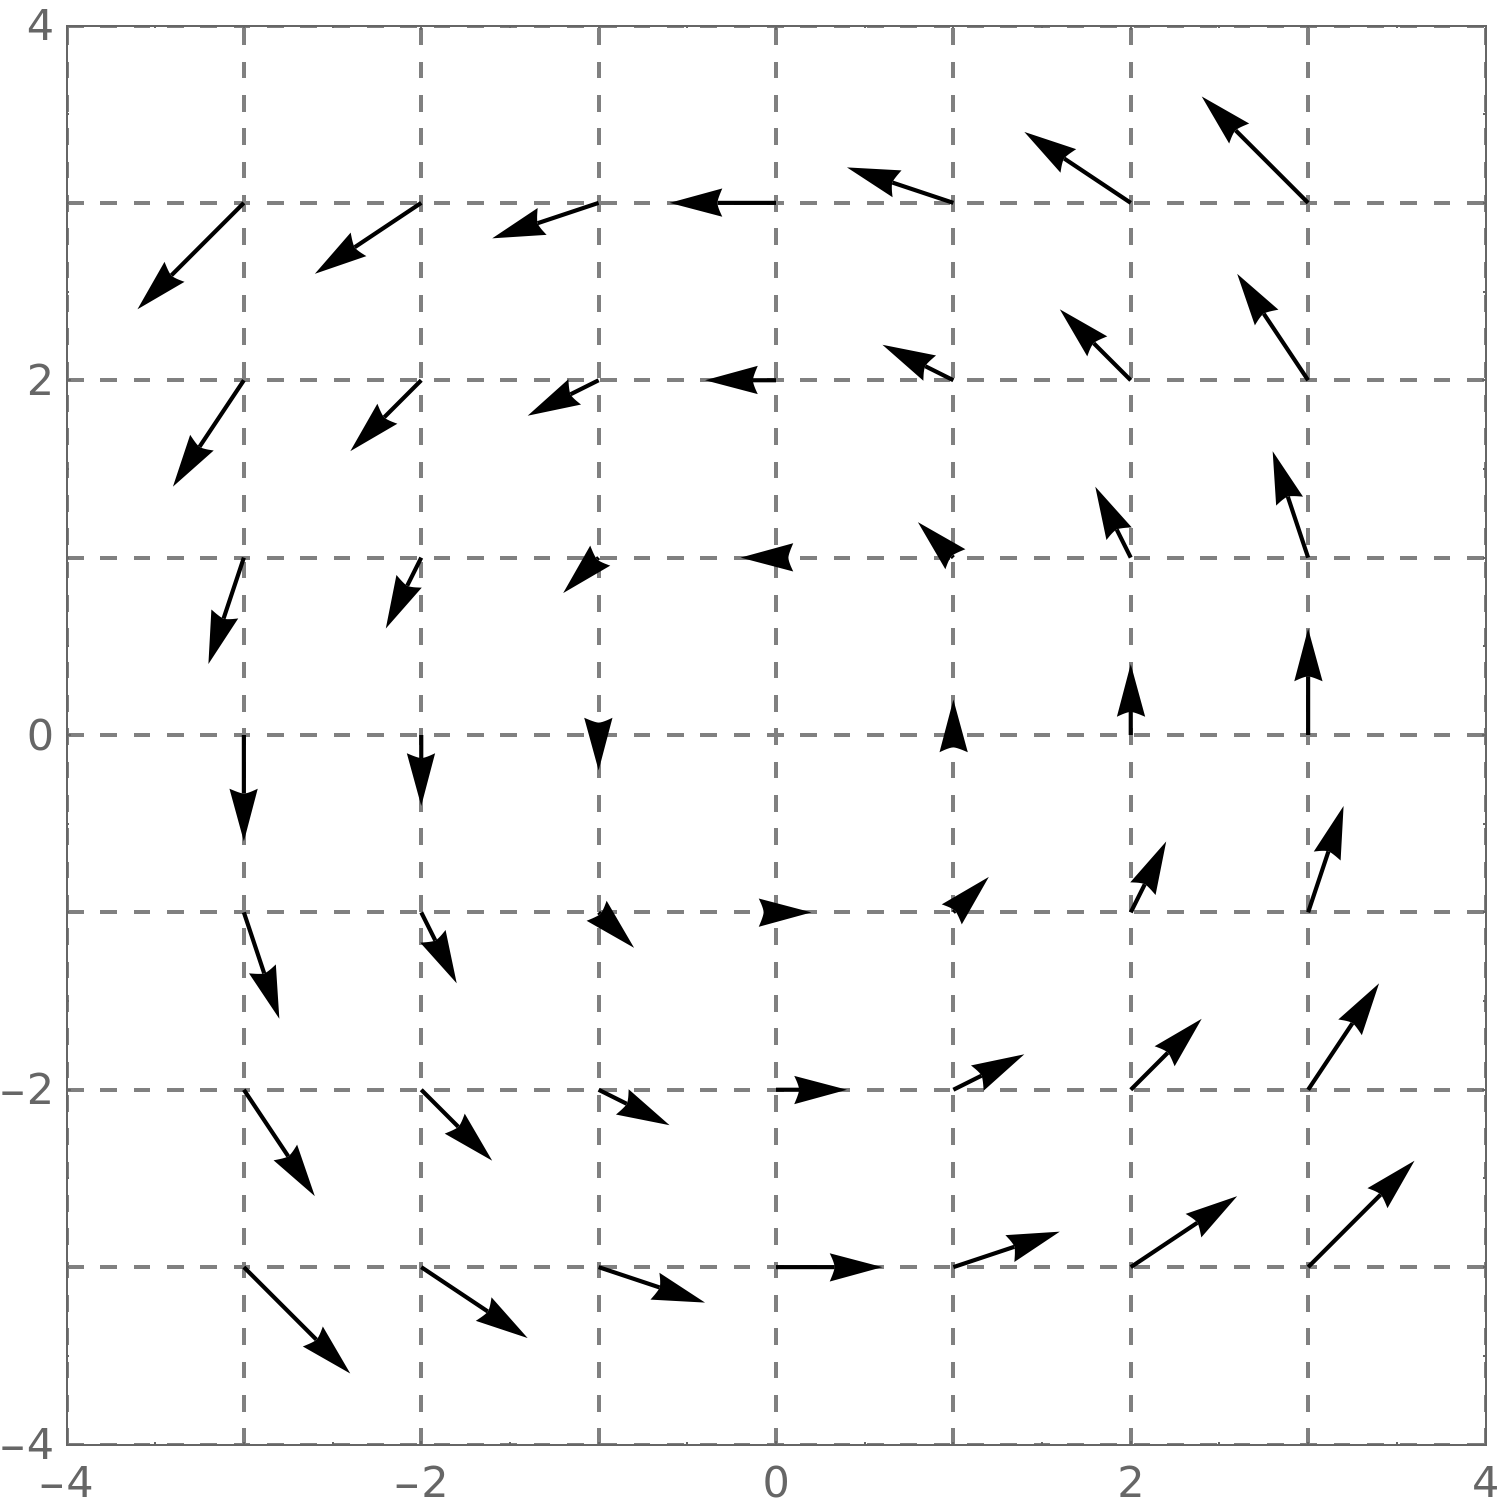
\includegraphics{rotField.png}
\end{image}

In essence, the scalar curl measures how the magnitude of the field
vectors change as you move to the right, in a direction perpendicular
to the direction of the field vectors:
\begin{image}
  \begin{tikzpicture}%[framed]
    \begin{axis}[
        hide axis,
        width=8cm,
        height=8cm,
        xmin=0,xmax=26,
        ymin=-12,ymax=24,
      ]
      \pgfplotsinvokeforeach{1,3,...,23}{
        \addplot[penColor,thick,->] coordinates{ (1,#1) (1,#1+1) };
      }

      \pgfplotsinvokeforeach{1,4,...,24}{
        \addplot[penColor,thick,->] coordinates{ (5,#1) (5,#1+2) };
      }

      \pgfplotsinvokeforeach{1,5,...,24}{
        \addplot[penColor,thick,->] coordinates{ (9,#1) (9,#1+3) };
      }

      \pgfplotsinvokeforeach{1,7,...,24}{
        \addplot[penColor,thick,->] coordinates{ (13,#1) (13,#1+5) };
      }

      \pgfplotsinvokeforeach{1,9,...,24}{
        \addplot[penColor,thick,->] coordinates{ (17,#1) (17,#1+7) };
      }

      \pgfplotsinvokeforeach{1,13,...,24}{
        \addplot[penColor,thick,->] coordinates{ (21,#1) (21,#1+11) };
      }
            
      \addplot[penColor,thick,->] coordinates{ (25,1) (25,24) };
 
       
       \node[inner sep=0pt,text width=7cm,scale=.9] at (axis cs:
       13,-6) {\footnotesize Since the magnitude of the field vectors
         \textbf{increases} as we move to the right, perpendicularly
         to the direction of the field vectors, the scalar curl is
         \textbf{positive.}};

    \end{axis}
  \end{tikzpicture}
\end{image}
And:
\begin{image}
  \begin{tikzpicture}%[framed]
    \begin{axis}[
        hide axis,
        width=8cm,
        height=8cm,
        xmin=0,xmax=26,
        ymin=-12,ymax=24,
      ]
      \pgfplotsinvokeforeach{1,3,...,23}{
        \addplot[penColor,thick,->] coordinates{ (25,#1) (25,#1+1) };
      }

      \pgfplotsinvokeforeach{1,4,...,24}{
        \addplot[penColor,thick,->] coordinates{ (21,#1) (21,#1+2) };
      }

      \pgfplotsinvokeforeach{1,5,...,24}{
        \addplot[penColor,thick,->] coordinates{ (17,#1) (17,#1+3) };
      }

      \pgfplotsinvokeforeach{1,7,...,24}{
        \addplot[penColor,thick,->] coordinates{ (13,#1) (13,#1+5) };
      }

      \pgfplotsinvokeforeach{1,9,...,24}{
        \addplot[penColor,thick,->] coordinates{ (9,#1) (9,#1+7) };
      }

      \pgfplotsinvokeforeach{1,13,...,24}{
        \addplot[penColor,thick,->] coordinates{ (5,#1) (5,#1+11) };
      }
            
      \addplot[penColor,thick,->] coordinates{ (1,1) (1,24) };
 
       
       \node[inner sep=0pt,text width=7cm,scale=.9] at (axis cs:
       13,-6) {\footnotesize Since the magnitude of the field vectors
         \textbf{decreases} as we move to the right, perpendicularly
         to the direction of the field vectors, the scalar curl is
         \textbf{negative.}};

    \end{axis}
  \end{tikzpicture}
\end{image}


In our next example, we see a field that has local rotation (nonzero
curl) but does not have global rotation.

\begin{example}
  Consider the following vector field $\vec{F}$:
      \begin{image}
        \begin{tikzpicture}
          \begin{axis}%
            [
	      ymin=-2.2,ymax=2.2,
	      xmin=-3.2,xmax=3.2,
              axis lines =middle, xlabel=$x$, ylabel=$y$,
              every axis y label/.style={at=(current axis.above origin),anchor=south},
              every axis x label/.style={at=(current axis.right of origin),anchor=west},
              grid=both,
              grid style={dashed, gridColor},
              xtick={-3,...,3},
              ytick={-2,...,2},
	    ]
            \pgfplotsinvokeforeach{-2,...,2}{
              \fill[penColor] (axis cs:0,#1) circle (2pt);
              }
            \pgfplotsinvokeforeach{-2,...,1}{
              \addplot[penColor,thick,->] coordinates{
                (1,#1+.05) (1,#1+.95) 
              };
            }
            \pgfplotsinvokeforeach{-2,...,1}{
              \addplot[penColor,thick,->] coordinates{
                (-1,.95 + #1) (-1,#1+.05) 
              };
            }
            \pgfplotsinvokeforeach{-2,0}{
              \addplot[penColor,thick,->] coordinates{
                (2,#1+.05) (2,#1+1.95) 
              };
            }
            \pgfplotsinvokeforeach{-2,0}{
              \addplot[penColor,thick,->] coordinates{
                (-2,1.95 + #1) (-2,#1+.05) 
              };
            }
            \addplot[penColor,thick,->] coordinates{
                (3,-1.5) (3,1.5) 
              };
            \addplot[penColor,thick,->] coordinates{
                (-3,1.5) (-3,-1.5) 
            };

            \fill[black,draw=black] (axis cs:2,1) circle (2.5pt);

            \node[right] at (axis cs:2,1) {$\vec{a}$};
              %% \node[inner sep=0pt,text width=8cm,right,scale=.85] at (axis cs:-6,-3.5)
              %%      {\footnotesize One should imagine a vector at
              %%        \textbf{every} point. We'll assume that the magnitudes
              %%        of the vectors are constant along horizontal lines.};
          \end{axis}
        \end{tikzpicture}
      \end{image}
      Setting $\d x = 1$ and $\d y = 1$, estimate:
      \[
      \curl \vec{F}(\vec{a})
      \]
      \begin{explanation}
        First note that one should imagine a vector at \textbf{every}
        point. We'll assume that the magnitudes of the vectors are
        constant along vertical lines. Set $\vec{F}(x,y) =
        \vector{M(x,y),N(x,y)}$. To estimate $\pp[N]{x}$, we examine
        the change in $N(x,1)$ between $x=1$ and $x=2$:
        \[
        \frac{N(2,1) - N(1,1)}{2-1} = \answer[given]{1}
        \]
        and we should also check the change of $N(x,1)$ between $x=2$
        and $x=3$:
        \[
        \frac{N(3,1) - N(2,1)}{3-2} = \answer[given]{1}
        \]
        Averaging these values together we find
        \[
        \pp[N]{x} \approx \answer[given]{1}
        \]
        To estimate $\pp[M]{y}$, we examine the change in $M(2,y)$
        between $y=0$ and $y=1$:
        \[
        \frac{M(2,1) - M(2,0)}{1-0} = \answer[given]{0}
        \]
        and we should also check the change of $M(2,y)$ between $y=1$
        and $y=2$:
        \[
        \frac{M(2,2) - M(2,1)}{2-1} = \answer[given]{0}
        \]
        Averaging these values together we find
        \[
        \pp[M]{y} \approx \answer[given]{0}
        \]
        So we approximate
        \[
        \curl\vec{F}(\vec{a})\approx\answer[given]{1}.
        \]
        So field above example does not have global rotation, but it
        does have local rotation.
      \end{explanation}
\end{example}

Now we'll show you a field that has global rotation but no local rotation!

\begin{example}
  Consider the vector field
  \[
  \vec{F}(x,y) = \vector{\frac{-y}{x^2+y^2},\frac{x}{x^2+y^2}}
  \]
  \begin{image}
    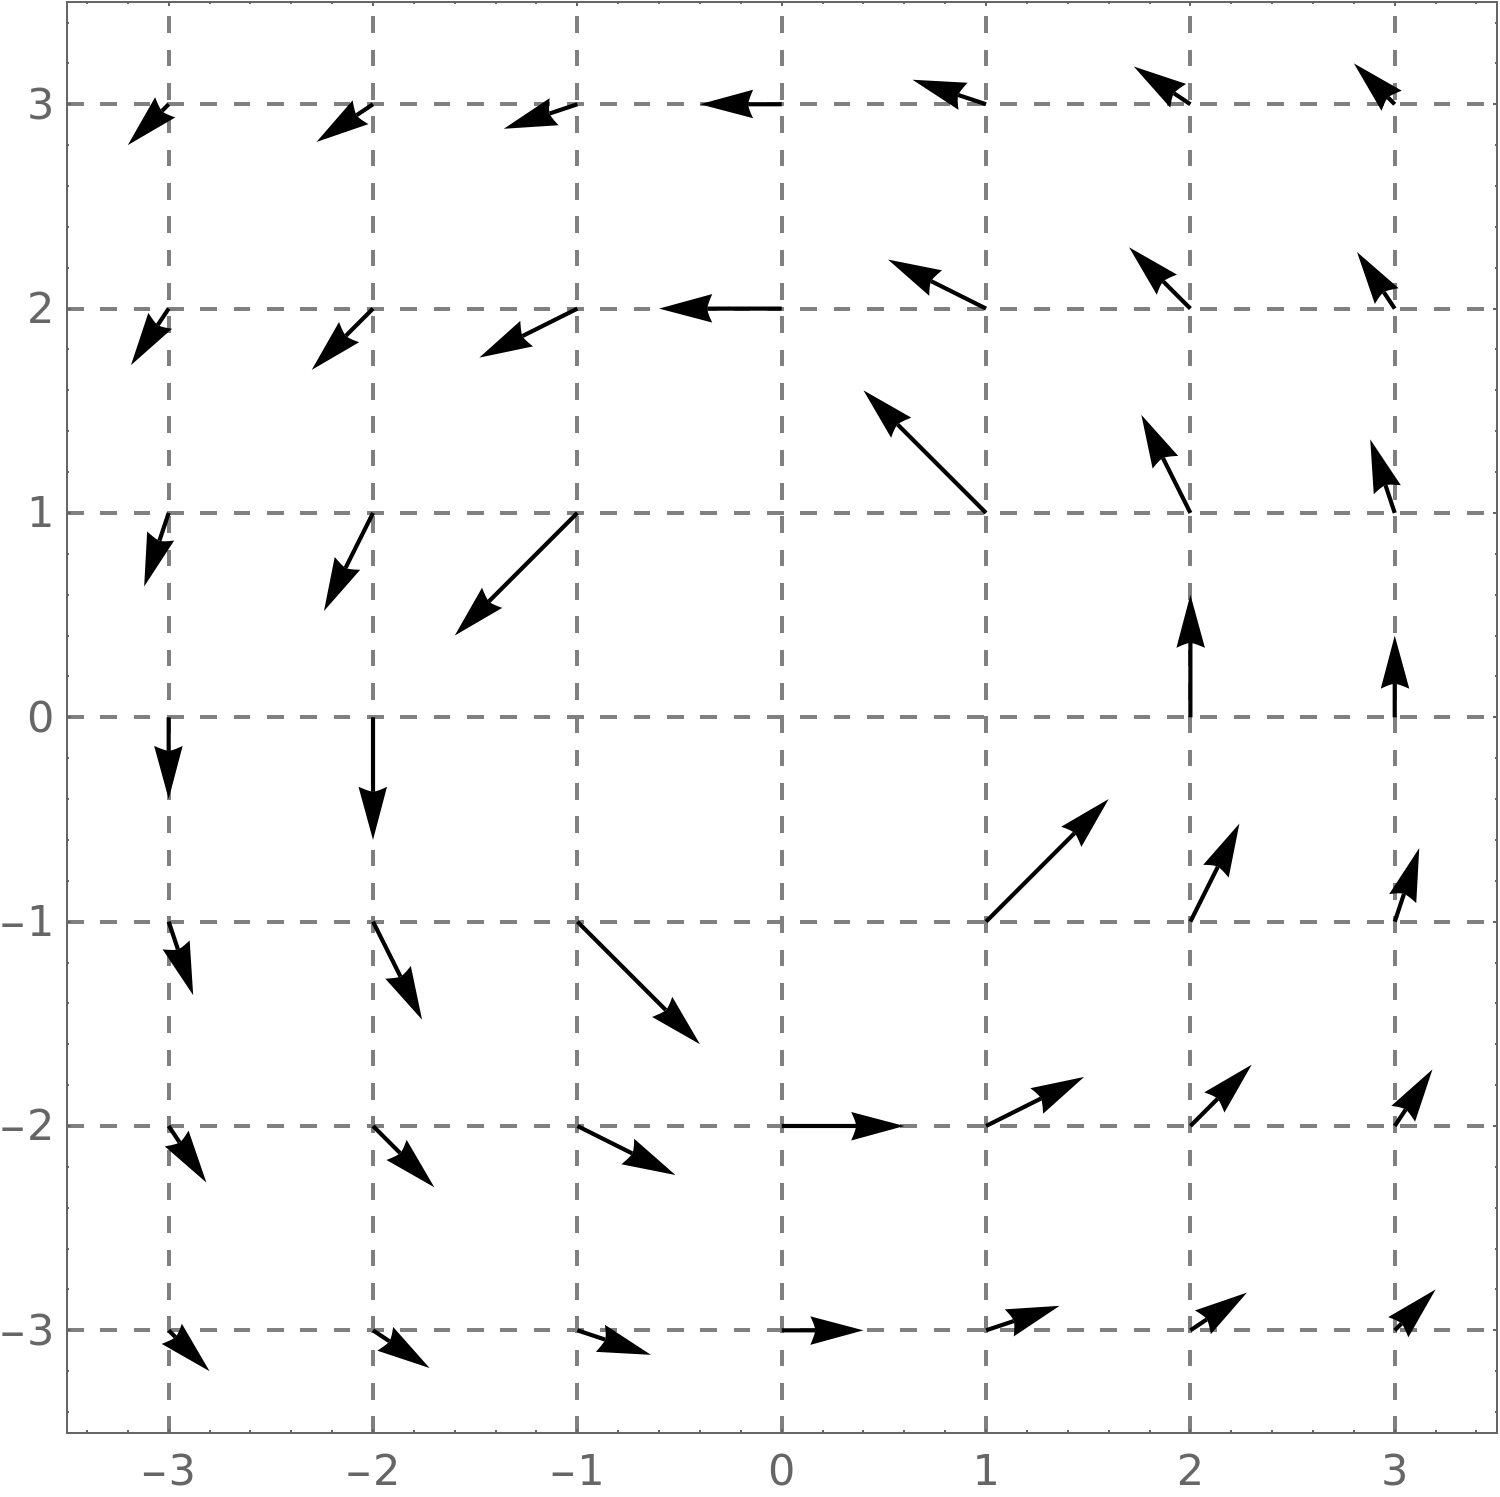
\includegraphics{rotFieldNot.png}
  \end{image}
  Compute:
  \[
  \curl\vec{F}(x,y)
  \]
  \begin{explanation}
    In this case, $\curl\vec{F}(x,y) =\answer[given]{0}$ when
    $\vector{x,y}\ne \vec{0}$. At $\vec{0}$, the curl of the vector
    field is \wordChoice{\choice{zero}\choice{infinity}\choice[correct]{undefined}},
    and hence this field is not a gradient field.  This field has
    global rotation, but it does not have local rotation.
  \end{explanation}
\end{example}

Finally, we'll show you a field that has global rotation with local
rotation in the \textit{opposite} direction!
\begin{example}
  Consider the vector field
  \[
  \vec{F}(x,y) = \vector{\frac{-y}{(x^2+y^2)^{3/2}},\frac{x}{(x^2+y^2)^{3/2}}}
  \]
  \begin{image}
    \includegraphics{oppoRotField.png}
  \end{image}
  Compute:
  \[
  \curl\vec{F}(x,y)
  \]
  \begin{explanation}
    In this case,
    \[
    \curl\vec{F}(x,y) =\answer[given]{\frac{-1}{(x^2+y^2)^{3/2}}}
    \]
    when $\vector{x,y}\ne \vec{0}$. Note, this is
    \wordChoice{\choice{positive}\choice[correct]{negative}} for all
    values of $x$ and $y$. This corresponds to local rotation in the
    \wordChoice{\choice[correct]{clockwise}\choice{counterclockwise}}
    direction.  This field has global rotation in the
    \wordChoice{\choice{clockwise}\choice[correct]{counterclockwise}}
    direction, but has local rotation in the
    \wordChoice{\choice[correct]{clockwise}\choice{counterclockwise}}
    direction.
  \end{explanation}
\end{example}


\subsection{Curl in three dimensions}

In this section we introduce curl in three dimensions. You already know how to compute it:
\begin{align*}
  \curl \vec F &= \det
  \begin{bmatrix}
    \veci & \vecj & \veck \\
    \pp{x} & \pp{y} & \pp{z}\\
    U & V & W
  \end{bmatrix}\\
  &= \veci\left(\pp[W]{y}-\pp[V]{z}\right)-
  \vecj\left(\pp[W]{x}-\pp[U]{z}\right)+
  \veck\left(\pp[V]{x}-\pp[U]{y}\right).
\end{align*}
What does it mean? Well first of all, in three dimensions, curl is a \textit{vector}. It points along the axis of rotation for a vector field. You should think of a tornado:
\begin{image}%% https://commons.wikimedia.org/wiki/File:Occluded_mesocyclone_tornado5_-_NOAA.jpg
  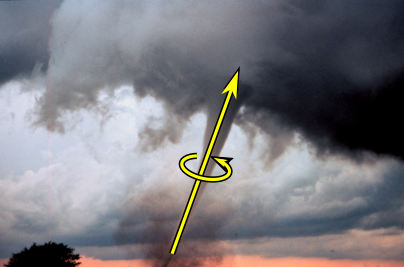
\includegraphics{tornado.png}
\end{image}
Here the vector pointing up is supposed to be the curl of the tornado.






At this point we only know how to take the derivative (via the curl)
of a vector field of two or three dimensions.  You can take another
course to learn more about derivatives of $n$-dimensional vector
fields.







\section{A new fundamental theorem of calculus}

Recall that a fundamental theorem of calculus says something like:
\begin{quote}
  To compute a certain sort of integral over a region, we may do a
  computation on the boundary of the region that involves one fewer
  integrations.
\end{quote}
In the single variable case we have:
\begin{image}
  \begin{tikzpicture}
    \node[inner sep=0pt] at (0,0) {$\int_a^b f'(x) \d x \quad = \quad f(b) - f(a)$};

    \node at (-1.5,-.7) {$\underbrace{\hspace{5.8em}}$};

    \node at (1.5,-.7) {$\underbrace{\hspace{5.5em}}$};

    \node[below,inner sep=0pt,text width=4cm,scale=.5] at (-1.65,-1) {To compute the signed area between $f'$ and the $x$-axis on the interval $[a,b]$,};

    \node[below,inner sep=0pt,text width=4cm,scale=.5] at (1.65,-1) {we can compute the difference in the values of $f$ when evaluated on the boundary.};
  \end{tikzpicture}
\end{image}
With line integrals we have:
\begin{image}
 \begin{tikzpicture}
    \draw [ultra thick, gray] plot [smooth] coordinates {(-2,2) (0,3) (-.5,2) (2,3)};
    \draw [ultra thick, gray,->,opacity=1] plot [smooth] coordinates {(0,2.9) (-.35,2.4)};
    \draw[black,fill=black] (-2,2) circle (.5ex);
    \draw[black,fill=black] (2,3) circle (.5ex);
    \node[black,left] at (-2,2) {$\vec{a}$};
    \node[black,right] at (2,3) {$\vec{b}$};
    \node[inner sep=0pt] at (0,1) {$\int_C \grad F \dotp  \d \vec{p}\quad= \quad F(\vec{b}) - F(\vec{a})$};

    \node at (-1.5,.3) {$\underbrace{\hspace{5.5em}}$};

    \node at (1.4,.3) {$\underbrace{\hspace{5.5em}}$};

    \node[below,inner sep=0pt,text width=4cm,scale=.5] at (-1.5,0)
         {To compute the accumulation of $\grad F$ along a curve $C$
           starting at $\vec{a}$ and ending at $\vec{b}$,};

    \node[below,inner sep=0pt,text width=4cm,scale=.5] at (1.5,0) {we can compute the difference in the values of $F$ when evaluated on the boundary.};
  \end{tikzpicture}
\end{image}
We now introduce a new fundamental theorem of calculus involving the
curl. It's called \textit{Green's Theorem}:

\begin{theorem}[Green's Theorem]\index{Green's Theorem}
  If the components of $\vec{F}:\R^2\to\R^2$ have continuous partial
  derivatives on a closed region $R$ where $C$ is a boundary of $R$
  and $\vec{p}(t)$ parameterizes $C$ in a counterclockwise direction
  with the interior on the left,
  \begin{image}
    \begin{tikzpicture}
      \draw[ultra thick, black,fill=gray] plot [smooth cycle] coordinates {(-1.5,.5) (.5,1) (1,2.5) (-1,2.5) (-2,1.5)};
      \draw[ultra thick,black, ->] plot [smooth] coordinates {(.85,1.51) (1.02,1.95)};
      \node[black] at (-.5,1.5) {$R$};
      \node[black,right] at (.5,1) {$C$};
    \end{tikzpicture}
  \end{image}
  then
  \[
  \iint_R \curl\vec{F}\d A = \oint_C \vec{F}\dotp\d\vec{p} 
  \]
\end{theorem}

\begin{example}
  Let $C$ be the rectangle with corners $(2,-1)$, $(2,4)$, $(3,4)$, and $(3,-1)$. Compute:
  \[
  \oint_C \frac{\sin(x)}{x} \d x + x^2 \d y
  \]
  \begin{explanation}
    We'll use Green's Theorem to squash this scary integral with
    ease. First note that if we imagine
    \[
    \oint_C \frac{\sin(x)}{x} \d x + x^2 \d y = \oint_C\vec{F}\dotp\d\vec{p}
    \]
    we set:
    \[
    \vec{F}(x,y) = \vector{\answer[given]{\frac{\sin(x)}{x}},\answer[given]{x^2}}
    \]
    Further note that our field is continuous on the interior of the
    rectangle. Thus we may apply Green's Theorem! Write with me now, 
    \[
    \curl \vec{F}(x,y) = \answer[given]{2x}
    \]
    So by Green's Theorem
    \[
    \oint_C \frac{\sin(x)}{x} \d x + x^2 \d y = \int_{\answer[given]{-1}}^{\answer[given]{4}}\int_{\answer[given]{2}}^{\answer[given]{3}} \answer[given]{2x}\d x\d y
    \]
    Now, keep writing with me,
    \begin{align*}
      \int_{\answer[given]{-1}}^{\answer[given]{4}}\int_{\answer[given]{2}}^{\answer[given]{3}} \answer[given]{2x}\d x\d y &= \int_{\answer[given]{-1}}^{\answer[given]{4}} \answer[given]{5} \d y\\
      &= \answer[given]{25}.
    \end{align*}
    The upshot is that we were able to use Green's Theorem to
    transform a tedious integral into a trivial one.
  \end{explanation}
\end{example}




\begin{question}
  Suppose that the curl of a vector field $\vec{F}:\R^2\to\R^2$ is
  constant, $\curl\vec{F} = 3$.
  \begin{image}
    \begin{tikzpicture}
      \begin{axis}%
        [
	  ymin=-3,ymax=5,
	  xmin=-8,xmax=4,
          axis lines =middle, xlabel=$x$, ylabel=$y$,
          every axis y label/.style={at=(current axis.above origin),anchor=south},
          every axis x label/.style={at=(current axis.right of origin),anchor=west},
          grid=both,
          grid style={dashed, gridColor},
          xtick={-10,...,4},
          ytick={-6,...,6},
	]
        \addplot[penColor2,ultra thick,smooth] coordinates{
          (-6,3) (-1,3) (-1,1) (2,1) (2,-1)
        };

        \addplot[penColor4,ultra thick,smooth] coordinates{
          (2,-1) (-4,-1) (-4,1) (-6,1) (-6,3)
        };

        \addplot[penColor2,ultra thick,->] coordinates{
          (-1.05,1.5) (-1,1.7) 
        };

        \addplot[penColor4,ultra thick,->] coordinates{
          (-4,.6) (-4.1,.4) 
        };

        \fill[black,draw=black] (axis cs:-6,3) circle (2.5pt);

        \fill[black,draw=black] (axis cs:2,-1) circle (2.5pt);
        \node[above,penColor2] at (axis cs:-3,3) {$C_1$};
        \node[below,penColor4] at (axis cs:-2,-1.05) {$C_2$};
        
      \end{axis}
    \end{tikzpicture}
  \end{image}
  If
  \[
  \int_{C_1} \vec{F} \dotp\d \vec{p} = 20
  \]
  estimate
  \[
  \int_{C_2} \vec{F}\dotp\d\vec{p}
  \begin{prompt}
    = \answer{46}
  \end{prompt}
  \]
  \begin{hint}
    Use Green's Theorem.
  \end{hint}
\end{question}


How is Green's Theorem a fundamental theorem of calculus? Well
consider this:
\begin{image}
  \begin{tikzpicture}
    \node[inner sep=0pt] at (0,0) {$\iint_R \curl\vec{F}\d A\quad =\quad \oint_C \vec{F}\dotp\d\vec{p}$};

    \node at (-1.3,-.7) {$\underbrace{\hspace{5.7em}}$};

    \node at (1.7,-.7) {$\underbrace{\hspace{5em}}$};

    \node[below,inner sep=0pt,text width=4cm,scale=.5] at (-1.3,-1)
         {To compute the double integral of $\curl \vec{F}$ over a
           region $R\subseteq\R^2$ with boundary $C$, };

    \node[below,inner sep=0pt,text width=4cm,scale=.5] at (1.8,-1) {we can compute the accumulation of $\vec{F}$ along a boundary curve $C$.};
  \end{tikzpicture}
\end{image}
The ``hand-wavey'' reason this works is given by the picture below:
\begin{image}
  \includegraphics{circulation.png}
\end{image}
Basically, $\curl \vec{F}\d A$ measures the circulation (local
rotation) in every little triangle above. Lining each of these little
triangles up, we see that the accumulation of this circulation is
measured by the flow of the vector field along the boundary, and this
is measured by:
\[
\oint_C \vec{F}\dotp\d\vec{p}
\]
Green's Theorem is our shiny new fundamental theorem of calculus. We'll be talking about it in the next two sections too!

\subsection{Strategy for evaluating line integrals}

At this point we have three ways to evaluating two-dimensional line
integrals:
\begin{itemize}
\item Direct computation.
\item The Fundamental Theorem of Line Integrals.
\item Green's Theorem.
\end{itemize}
How do you know which method to use? Here are some rules of thumb.

\paragraph{Identify the field}
With line integrals, we must have a vector field. You must identify this vector field. 


\paragraph{Compute the scalar curl of the field}
If the scalar curl is zero, then the field is a gradient field.
If the scalar curl is ``simple'' then proceed on, any you might want to use Green's Theorem.


\paragraph{Is the boundary  a closed curve?}
If the field is a gradient field and the curve is closed, then the
integral is zero (by both the Fundamental Theorem of Line Integrals
and Green's Theorem).

If the boundary is not a closed curve and the curl is not zero, you
must use direct computation.

If the curl is simple and the boundary is a closed curve, then maybe
use Green's Theorem.



\subsection{The shape of things to come}

Recalling that $C^\infty(A,B)$ is the set of differentiable functions
from $A$ to $B$ where \textbf{all} of the derivatives are continuous,
we can make the following ``chain'' of derivatives:

\[
\underbrace{C^{\infty}(\R^2,\R)}_{\text{surfaces}} \overset{\grad}{\to}\underbrace{C^\infty(\R^2,\R^2)}_{\text{vector fields}} \overset{\curl}{\to}\underbrace{C^\infty(\R^2,\R)}_{\text{surfaces}} 
\]
Moreover, by the Clairaut gradient test, the scalar curl of the
gradient vector is zero. Given a function $F:\R^2\to\R$, we can follow
$F$ through the chain to see what happens:
\begin{image}
  \begin{tikzpicture}
    \node{
    \begin{tikzcd}[ampersand replacement=\&,row sep=-.5em]
     C^{\infty}(\R^2,\R) \arrow[r,"\grad"] \& C^{\infty}(\R^2,\R^2) \arrow[r,"\curl"] \& C^{\infty}(\R^2,\R)\\
     F \arrow[r,mapsto] \& \grad F  \arrow[r,mapsto] \& 0
    \end{tikzcd}};
  \end{tikzpicture}
\end{image}
This is nothing more than a fancy way to say that $\curl\grad F =
0$. However, we also have our two new fundamental theorems of
calculus: The Fundamental Theorem of Line Integrals (FTLI), and
Green's Theorem. These theorems also fit on this sort of diagram:
\begin{image}
  \begin{tikzpicture}
    \node{
    \begin{tikzcd}[ampersand replacement=\&,row sep=-.5em]
     C^{\infty}(\R^2,\R) \arrow[r,"\grad"] \& \arrow[l,"\text{FTLI}",bend left=20 ]C^{\infty}(\R^2,\R^2) \arrow[r,"\curl"] \& \arrow[l,"\text{Green's Theorem}", bend left =20]C^{\infty}(\R^2,\R)
    \end{tikzcd}};
  \end{tikzpicture}
\end{image}
 The Fundamental Theorem of Line Integrals is in some sense about
 ``undoing'' the gradient. Green's Theorem is in some sense about
 ``undoing'' the scalar curl. Are there more fundamental theorems of
 calculus? Absolutely, read on young mathematician!



\end{document}
